\section{Program Logistics}

% Request review from Katy Huff
\subsection{Potential Speakers}

\subsubsection{Rachel Slaybaugh, UC Berkeley}
% \begin{wrapfigure}{r}{0.5\textwidth}
% 	\begin{center}
% 		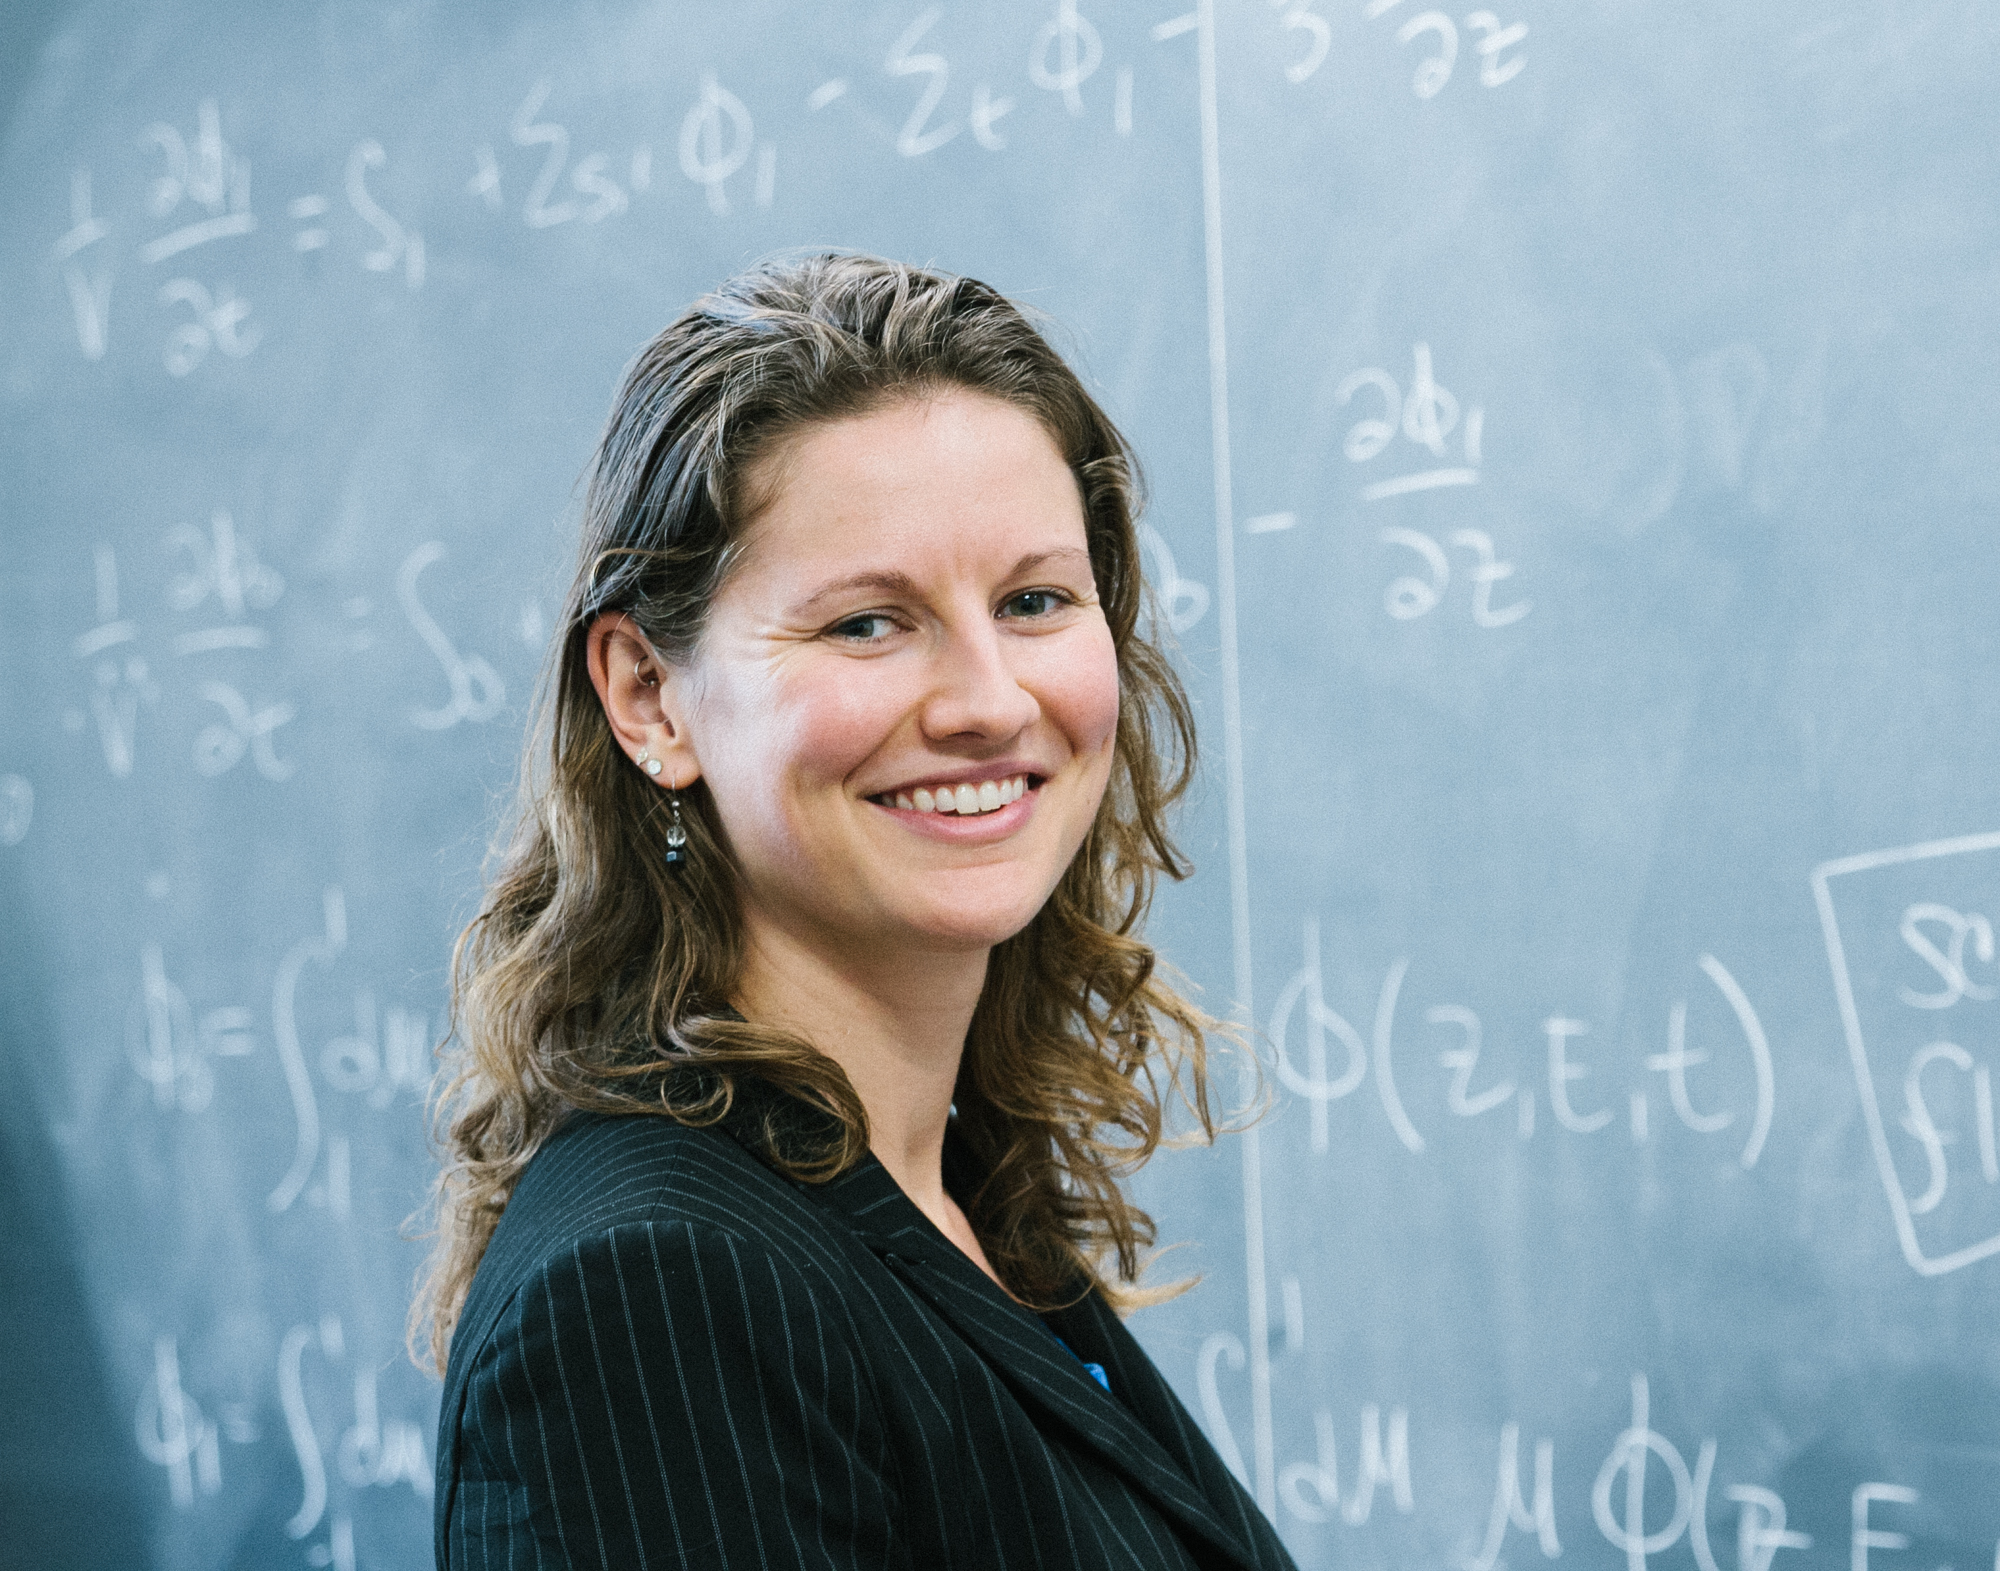
\includegraphics[width=0.48\textwidth,scale=0.2]{slaybaugh.jpg}
% 	\end{center}
% \end{wrapfigure}
Prof. Slaybaugh's research is based in numerical methods for neutron transport with an emphasis on supercomputing. She applies these methods to reactor design, shielding, and nuclear security and nonproliferation. Slaybaugh was a key founder of the nuclear innovation bootcamp, which seeks to train students and professionals in skills essential to innovation in nuclear energy while executing team projects. Finally, Slaybaugh has served as a Program Director at ARPA-E, developing and running their first fission energy programs. Advanced Research Projects Agency-Energy (ARPA-E) invests in research for ways to generate, use, and store energy. These projects have the potential to radically improve economic prosperity in the U.S. and environmental wellbeing. Due to her endeavors in teaching and sharing nuclear innovation, we believe that Slaybaugh's goals are aligned with the goals of this conference and would make her an excellent addition to the program. Slaybaugh has much to offer the conference with her vision and leadership.

\subsubsection{Suzanne Hobbs Baker}
% \begin{wrapfigure}{r}{0.5\textwidth}
% 	\begin{center}
% 		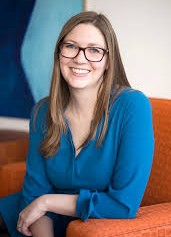
\includegraphics[scale=0.75]{hobbsbaker.jpeg}
% 	\end{center}
% \end{wrapfigure}
Talking about nuclear energy, specifically with the general public, is one of Suzanne Hobbs Baker's key goals. Baker has a strong track record as a nuclear science communicator. In 2008 she founded a nonprofit organization aimed at reaching women, minorities, and young people with critical information about climate change and nuclear energy. She currently works as the creative director for Fast Path to Zero Initiatve at the University of Michigan and as a Nuclear security fellow with Third Way Energy. Baker's work in empowering minorities and students to solve the world climate crisis with nuclear energy, as well as her skill in creative science communication, ensures that Baker has a lot to offer the student conference. Celebrating the people behind the science is one of the key goals of this conference and an area in which Baker has a lot of experience.

\subsubsection{Todd Allen, UW Madison}
% \begin{wrapfigure}{r}{0.5\textwidth}
% 	\begin{center}
% 		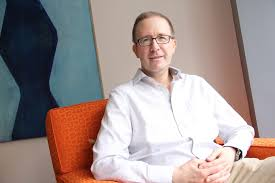
\includegraphics[scale=0.75,width=0.48\textwidth]{allen.jpeg}
% 	\end{center}
% \end{wrapfigure}
His first post-Ph.D. position was as a staff scientist at Argonne National Laboratory. While at Argonne, he joined the leadership team tasked with developing the Generation IV Roadmap, the document that framed the resurgence of the nuclear research programs early in the 21st Century.Following Argonne, he joined the faculty at the University of Wisconsin. While there, he split his time between establishing a premier material science program at the university and supporting the Idaho National Laboratory. At INL, he led the transition of the Advanced Test Reactor into a national user facility. He also ran a six-institution Energy Frontier Research Center focused on answering fundamental questions about heat transfer in nuclear fuel.
From 2013-2016, he helped lead the Idaho National Laboratory as the Deputy Laboratory Director for Science $\&$ Technology, including being an important contributor to the development of the Gateway for Accelerated Innovation in Nuclear (GAIN) initiative announced at the White House in November 2015. Since 2016 he has been a Visiting Senior Fellow with Clean Energy Program at Third Way, a Washington, DC based think tank. His role in formulating the roadmap for Generation IV reactors and his leadership indicate that he would make a great speaker at the conference.

\subsubsection{Rita Baranwal, DOE Nuclear Energy}
Dr. Rita Baranwal serves as the Assistant Secretary for the Office of Nuclear Energy in the U.S. Department of Energy (DOE).  Dr. Baranwal leads the office’s efforts to promote research and development (R$\&$D) on existing and advanced nuclear technologies that sustain the existing U.S. fleet of nuclear reactors, enable the deployment of advanced nuclear energy systems, and enhance the U.S.A.'s global commercial nuclear energy competitiveness. Prior to her current role, Dr. Baranwal directed the Gateway for Accelerated Innovation in Nuclear (GAIN) initiative at Idaho National Laboratory.  She was responsible for providing the nuclear industry and other stakeholders access to DOE's state-of-the-art R$\&$D expertise, capabilities, and infrastructure to achieve faster and cost-effective development, demonstration, and ultimate deployment of innovative nuclear energy technologies. Under her leadership, GAIN positively impacted over 120 companies. Baranwal is a clear choice of speaker to discuss the ways to improve nuclear legislation and how companies can rapidly develop new nuclear technology.


\subsubsection{Jim Conca, Forbes}
Jim Conca has been a scientist in the field of the earth and environmental sciences for 33 years, specializing in geologic disposal of nuclear waste, energy-related research, planetary surface processes, radiobiology and shielding for space colonies, subsurface transport and environmental clean-up of heavy metals. He is a Trustee of the Herbert M. Parker Foundation, Adjunct at WSU, an Affiliate Scientist at LANL and consult on strategic planning for the DOE, EPA/State environmental agencies, and industry including companies that own nuclear, hydro, wind farms, large solar arrays, coal and gas plants. He also writes for Forbes magazine about nuclear issues, energy, and the environment. Conca has a strong vision for the future and is not shy about coming up with ideas to solve grand challenge problems. In addition to his experience and ambition, he is an excellent science communicator to scientists and non-scientists alike. Together, these factors make him an ideal speaker at the conference.

\subsubsection{Fatima Ebrahimi, Princeton}
Fatima Ebrahimi is a Research Physicist at the PPPL Theory Department
and an Affiliated Research Scholar at the Department of Astrophysical
Sciences, Princeton University. She has many years of experience in theoretical and global computational extended magnetohydrodynamics (MHD) with wide applications to laboratory fusion and astrophysical plasmas. Her main research interests are MHD
stability in fusion plasmas, momentum transport, dynamos, and magnetic reconnection in laboratory fusion and astrophysical plasmas. She has written many papers over a wide range of topics and peer-reviewed journals. She is an elected executive committee member
of the APS Topical Group in Plasma Astrophysics (GPAP), 2018-2021, and program committee member for U.S. Magnetic Fusion Research (MFR) Strategic Directions, 2017-2018. Dr. Ebrahimi is a great choice to have as a speaker on the future of fusion energy. 

\subsubsection{Brian Jurczyk, CEO Starfire Industries}
Brian holds a dual PhD/MBA degree with background in aerospace, nuclear, plasma and radiological engineering and technology commercialization.  As CEO, Brian works to find creative win-win solutions with commercial and industrial partners for particularly challenging applications - at all stages of value creation from basic IP development through early-stage manufacturing.  In 2012-13, Brian received the Innovation Celebration "Entrepreneurial Excellence in Management Award," was named to Central Illinois Business' "40-under-40" and has served as Chairperson of the Champaign-Urbana CEO Roundtable. As a professional leader in plasma and radiological engineering, Jurczyk would be a great speaker to have at the conference on topics related to the future of plasma engineering and professional development.

\subsection{Panels}

